\begin{table}[H]
	\centering
	\caption[short title]{main title}\label{tab:table}
	\begin{threeparttable}
	\arrayrulecolor{gray}
		\begin{tabular}{|m{0.5\linewidth}|m{0.5\linewidth}|}
			\hline
			\rowcolor{gray}
			\small\textcolor{white}{\textbf{Modul}} & \small\textcolor{white}{\textbf{Aufgabe}} \\
			\hline
			. & .\\
			\hline
			. & .\\
			\hline
		\end{tabular}
		\begin{tablenotes}
			\tiny
			\item tablenotes here!
		\end{tablenotes}
	\end{threeparttable}
\end{table}

\begin{figure}[h]
	\centering
	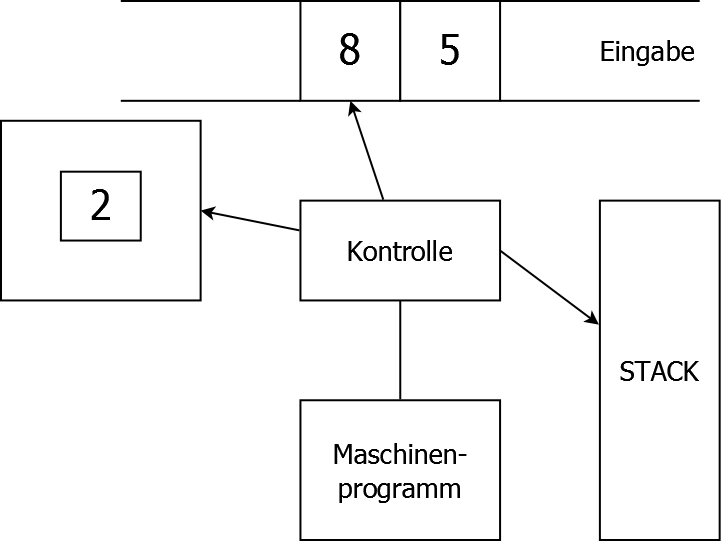
\includegraphics[width=300px]{gfx/architecture.png}
\end{figure}